\documentclass[11pt]{amsart}
\usepackage[margin=1in]{geometry}
\usepackage{graphicx}
\usepackage{siunitx}
\usepackage{amsmath,amsfonts,amsthm,amssymb,amsaddr}
\usepackage{hyperref}
\usepackage{fancyhdr}
\usepackage{multicol, caption}
\newenvironment{Figure}
  {\par\medskip\noindent\minipage{\linewidth}}
  {\endminipage\par\medskip}

\graphicspath{ {./images/} }

%\makeatletter
%\def\subsection{\@startsection{subsection}{3}%
%  \z@{.5\linespacing\@plus.7\linespacing}{.1\linespacing}%
%  {\normalfont\itshape}}
%\makeatother

\title{Lab Report}

\author{Joe Bentley}

\address{School of Physics and Astronomy \\ Tutor: Kevin Ralley}
\email{joebentley10@gmail.com}

\date{\today}

\begin{document}

\begin{abstract}
  In this paper the higgs data is analysed and we find the higgs with this statistical significance etc.
\end{abstract}

\maketitle

\newpage

\pagestyle{fancyplain}

\lhead{\footnotesize {Joe Bentley}}
\rhead{\footnotesize {Lab Report}}

\begin{multicols}{2}

\section{Theory}

\subsection{Four Momentum}
\label{sec:fourmomentum}

The four momentum is similar to the classical three component momentum except generalised to four dimensional space-time, so it also has an energy component. \cite{kinematics} In the data supplied the four-momentum is given in the form $(p_x, p_y, p_z, E)$, where $p_z$ is aligned along the beam axis

The transverse momentum is the component of the momentum perpendicular to the beam axis. Since the $z$ component of the four-momentum, $p_z$ is aligned along the beam axis, the transverse momentum is given by,

\begin{equation}
  \label{eq:transverse}
  p_T = \sqrt{{p_x}^2 + {p_y}^2}
\end{equation}

The pseudorapidity is a measure of the angle between the particle and the beam axis, and is defined as $\eta = -\ln{\left[\tan{\left(\frac{\theta}{2}\right)}\right]}$. This can be calculated from the cartesian momentum components using, (RELATE THIS TO RAPIDITY)

\begin{equation}
  \label{eq:pseudorapidity}
  \eta = \sinh^{-1} \frac{p_z}{p_T}
\end{equation}

The azimuthal angle is the angle subtended by the $x$ and $y$ momentum components, so the angle between the momentum components that are perpendicular to the beam axis, in contrast to the pseudorapidity, which is between the particle trajectory and the beam axis, (MAKE SENSE?) (DIAGRAM?)

\begin{equation}
  \label{eq:azimuthal}
  \phi = \tan^{-1} \frac{p_y}{p_x}
\end{equation}

\subsection{Higgs Decay Channels}

The Higgs can decay through a few different modes:

\begin{itemize}
    \item Fermion-antifermion pair
    \item Pair of massive gauge bosons
    \item Pair of massless gauge bosons (through heavy virtual quark or massive gauge boson loop)
\end{itemize}

\cite{decaymodes1} \cite{decaymodes2}

(MAYBE A BIT MORE EXPLANATION ABOUT THESE DECAY MODES?! (GET ANOTHER SOURCE?!)

The decay channel investigated in this experiment is the last one, the decay of the Higgs into two photons by a heavy virtual quark (top) or massive gauge boson (W boson) loop. This is significantly rarer than the other decay modes as seen in the small branching fraction of $0.0023$ (so it occurs twice in every thousand decays) \cite{HiggsCross1}, but is used because the momenta of the photons can be measured much more accurately than other more massive particles, since the momenta of the photon is directly proportional to its energy, as the photon has no rest mass. (GET SOURCE) (HOW TO MEASURE PARTICLE MOMENTUM? LOOK AT ATLAS EXPERIMENT)

\subsection{Invariant Mass}
\label{sec:invariant}

To find the mass of the particle(s) before a collision event, the invariant mass is used, which is the mass which remains unchanged through a Lorentz transform (GET SOURCE). The sum of the invariant masses of the products of an interaction is the same as the sum of the invariant masses of the original particles, so by calculating the invariant masses of the resultant particles of the collision events, we have calculated a series of invariant mass values corresponding to the inputs of the collision event. Since the Higgs invariant mass is known (ROUGHLY?!?), the frequency of values in that window should be higher.

The invariant mass is calculated using the relativistic equation for energy, in natural units this is given by,

\begin{equation}
  \label{eq:invariantmass}
  m_0^2 = E^2 - {|\mathbf{p}|}^2
\end{equation}

This is calculated in the parsing program by summing the four momenta from the event and then taking the scalar product of the resulting vector with itself. Minkowski space-time has signature $(+, -, -, -)$ so the scalar product has the effect of the above equation. We then take the square root of the scalar product to find the invariant mass. \cite{kinematics}

The mass window is taken to be $\SI{115}{\giga\electronvolt}$ to $\SI{135}{\giga\electronvolt}$, which is roughly $\pm \SI{10}{\giga\electronvolt}$ the expected Higgs mass, as measured. \cite{Higgs}

\section{PYTHIA}
\label{sec:pythia}

The GPL-licensed PYTHIA was used to generate the collision data used in this experiment. \cite{pythia} The event data is given in a flat text file format. The file consists of a series of events, which start with a header ``Event $n$'', the subsequent lines are the four momenta of the products of the collision event, each line in the format ``$p_x$ $p_y$ $p_z$ $E$'', where $p_z$ is aligned along the beam axis. Then there is another line ``Event $n+1$'' with subsequent lines being four momenta events and so on.

\section{Programming}

The scripts used in this experiment were written in Python 3, and used the numpy (numeric Python) module for generating the histogram, and PyPlot (from matplotlib) for plotting the histogram and significance plots. Three different scripts are used in this experiment,

\subsection{parse.py}

The script parse.py parses the event data in the format described in section ~\ref{sec:pythia} into individual event objects which each contain a list of four momenta objects. In these event classes we have methods which do useful operations like calculating the invariant mass of the event using the four momenta. The four momenta class has methods that allow us to easily calculate the transverse momentum, azimuthal angle, and pseudorapidity, as well as allowing us to add and take the dot product of four momenta. The parsing scripts also contains the filters which are used to filter out Higgs events from background events, and are discussed in more depth in section ~\ref{sec:filters}. The invariant masses are calculated for each event in the event data file and then each invariant mass is written to a line in the output invariant masses file.

\subsection{significance.py}

This scripts optimises the filters used on the Higgs and background data by using a series of parameters with the filters and testing them on the entire data set; the significance is taken for the parameters and this is used to find the best filter parameters, as discussed in section ~\ref{sec:optimisation}. This script parses and filters the data using the parsing module.

\subsection{plot.py}

The plotting script generates the histogram of both the higgs and background event data together, called the combined mass histogram. The significance in the mass range (WHAT MASS RANGE) is calculated by counting the number of Higgs events in the mass range and the number of background events in the mass range and then using eq.~\ref{eq:significance} to calculate the statistical significance. The script can also generate an invariant mass plot from the combined mass histogram.

\section{Weighting}

The data given included $10,000$ signal events and $1,000,000$ background events. This is a much smaller ratio of signal to background events than would actually be observed in a real collider experiment, due to the low branching fraction of the $H \to \gamma\gamma$. The branching fraction is the fraction of all particles which decay through a given decay mode, in this case the fraction of $H \to \gamma\gamma$ decays over all Higgs decay modes. The theoretical ratio of the observed Higgs events to observed background events can be calculated by taking the ratio of the Higgs production cross section to the background cross section and multiplying it by the branching fraction of $H \to \gamma\gamma$,

\begin{equation}
  \label{eq:weighting}
  \frac{\text{num. H}}{\text{num. back}} = \frac{\sigma{\left(\text{H prod}\right)} \cdot B_f\left(H\to\gamma\gamma\right)}{\sigma{\left(\text{back}\right)}}
\end{equation}

where $\text{num. H}$ is the number of signal events, $\text{num. back}$ is the number of background events, $\sigma{\left(\text{H prod}\right)}$ is the Higgs production cross section, $\sigma{\left(\text{back}\right)}$ is the background cross section, and $B_f\left(H\to\gamma\gamma\right)$ is the branching fraction of Higgs to diphoton.

The branching fraction is given by $B_f\left(H\to\gamma\gamma\right) = 0.0023$, and the cross sections are given by $\sigma{\left(\text{H prod}\right)} = \SI{17.12}{\pico\barn}$, and $\sigma{\left(\text{back}\right)} = \SI{140}{\pico\barn}$. The Higgs cross section and branching fraction are taken at roughly the expected Higgs mass $\SI{125}{\giga\electronvolt}$, \cite{Higgs} where the cross section is taken from the ABPS calculation for $\sqrt{s} = \SI{14}{\tera\electronvolt}$ where $s$ is the center-of-momentum energy (the energy in the frame where the net momenta is zero). \cite{HiggsCross1} (MORE JUSTIFICATION NEEDED). The background cross section is taken from the PYTHIA collision event generator.


\section{Filters}
\label{sec:filters}

There are many more background events than there are from the signal (Higgs) events in our data. After the weighting, there are roughly $100$ Higgs events to $100,000,000$ background events, so in the combined invariant mass histogram the Higgs is practically invisible. Thus filtering needs to be applied for there to be any chance to be able to observe the Higgs in the invariant mass histogram. This is implemented in the form of event selection in which we attempt to remove the background data while retaining the Higgs data. A few types of filtering are used: number threshold, transverse momenta, energy, angular (azimuthal and pseudorapidity).

\subsection{Number}

The first filter applied a threshold to the number of four momenta in the collision event. It is required that the event must have at least two four momenta, as the $H \to \gamma\gamma$ will produce at least two photons, not just one.

\subsection{Transverse Momenta}

The transverse momenta is the component of the momentum perpendicular to the beam axis as described in section ~\ref{sec:fourmomentum}. This is filtered in two passes over both the signal and higgs events. Given an event with four momenta, first the event is discarded unless it has at least one four momentum above a given threshold, then all four momenta in the event below a certain threshold are discarded.

(JUSTIFICATION)

\subsection{Energy}

(Filter the energy, not sure if we will see results)

\subsection{Angular}

(Filter the difference in azimuthal angle and pseudorapidity squared)

\subsection{Final Selection}

There are two methods that were proposed to choose the final two transverse momenta to use to calculate the invariant mass. First it was decided to try an azimuthal angle based filter, where the most back-to-back photons (the photons with an azimuthal angle with the greatest difference) would be chosen to calculate the invariant mass. (WHY DIDN'T YOU DO THIS?!?) Instead all but the two highest transverse momenta photons are discarded, and the two remaining are used to calculated the invariant mass.


\section{Optimisation of Filters}
\label{sec:optimisation}

To find the filter parameters that give the best chance of finding the Higgs we used the formula for the statistical significance of the higgs,

\begin{equation}
  \label{eq:significance}
  \Sigma = \frac{\text{no. signal}}{\sqrt{\text{no. signal} + \text{no. background}}}
\end{equation}

Each filter is applied to the signal (Higgs) and background events and then the above equation is used to find the statistical significance of the Higgs in those events by counting the number of signal and background events left after filtering. To find the best parameters to use for the filters a range of different parameters are tested for each filter. For example for the transverse momenta filter, the threshold is originally applied from $\SI{0}{\giga\electronvolt}$ to $\SI{700}{\giga\electronvolt}$ in steps of $\SI{100}{\giga\electronvolt}$. The value that gives the best statistical significance is then chosen as the current candidate for the best optimised value. Then the value is further optimised by taking the currently best optimised value and then calculating the statistical significance for the values around it, for example checking the statistical significance at $\SI{\pm10}{\giga\electronvolt}$ the current value for the above example. After repeating this process a few times (HOW MANY TIMES?) the most optimum filter values to see the most Higgs event in the invariant mass histogram are found.

INCLUDE SIGNIFICANCE PLOT!!!


\section{Invariant Mass Histogram}

The numpy library is used to generate an combined (signal and background) invariant mass histogram from the invariant masses calculated in the parsing script. The statistical significance of the signal (Higgs) is calculated using eq.~\ref{eq:significance} over the mass window discussed in section ~\ref{sec:invariant}, and gives a measure of how sure we can be that it is the Higgs in this mass range.

\begin{Figure}
  \centering
  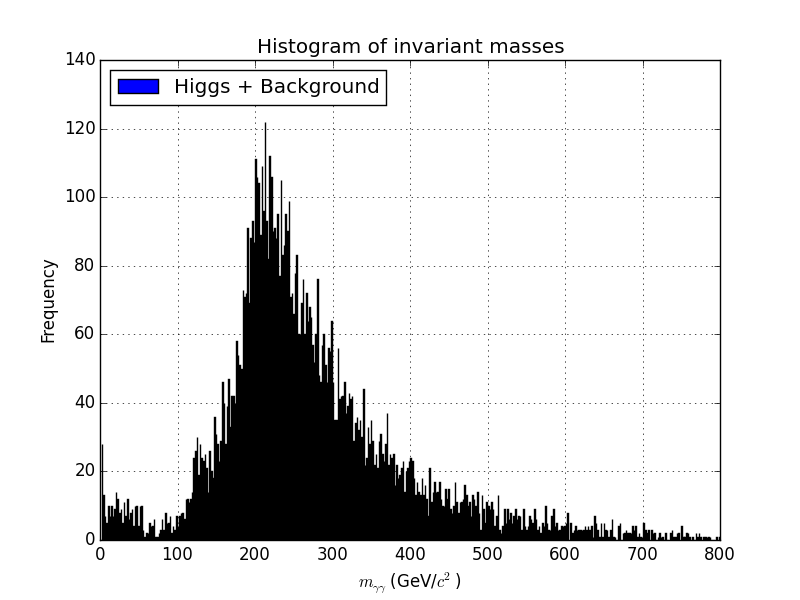
\includegraphics[width=\linewidth]{invmass}
  \captionof{figure}{Our awesome invariant mass plot yo!}
  \label{fig:invmass}
\end{Figure}

(DISCUSS RESULTS!!!)

\section{Results}

\end{multicols}

\bibliographystyle{plain}
\bibliography{citations}
\end{document}
